\section{ JavaScript}

\begin{frame}[fragile]{CH8 JavaScript}
\begin{figure}
    
\includegraphics[width=0.9\textwidth]{figure/javascript.jpg}
\end{figure}
\end{frame}

\begin{frame}[fragile]{本章学习目标}
\begin{easylist} \easyitem
& 了解JavaScript的起源
& 掌握JavaScript的测试方法
& 熟悉JavaScript的基本语法,能借助于文档进行基本的脚本编写
& 了解浏览器对象模型BOM
& 理解JavaScript的定时器操作
\end{easylist}
\end{frame}

\begin{frame}[fragile]{目录}
\begin{easylist} \easyitem
& JavaScript概述
& JavaScript的测试方法
& JavaScript的变量和常量
& JavaScript的基本语句
& 函数和数组
& 对象
& 浏览器对象模型BOM
& 定时器
\end{easylist}
\end{frame}


\subsection{8.1 JavaScript概述}

\begin{frame}[fragile]{8.1 JavaScript概述}
\begin{easylist} \easyitem
& 1995年 $\rightarrow$ Brendan Eich $\rightarrow$ 网景公司  $\rightarrow$ JavaScript
& JavaScript vs Applet
& JavaScript vs JScript
& 当前JavaScript的三大组成部分
&& ECMAScript语言核心
&& DOM(Document Object Model)文档对象模型
&& BOM(Browser Object Model)浏览器对象模型
\end{easylist}
\end{frame}


\begin{frame}[fragile]{jQuery}
\begin{easylist} \easyitem
& JavaScript的跨浏览器问题
& jQuery解决方案
&& John Resig创建的一个轻量级JavaScript库
&& 充分利用了CSS的优势,支持扩展,能够抽象浏览器的不一致性,并支持隐式迭代和连缀操作
\end{easylist}
\end{frame}


\begin{frame}[fragile, allowframebreaks]{jQuery}
\begin{easylist} \easyitem
& 下载使用
\begin{figure}
    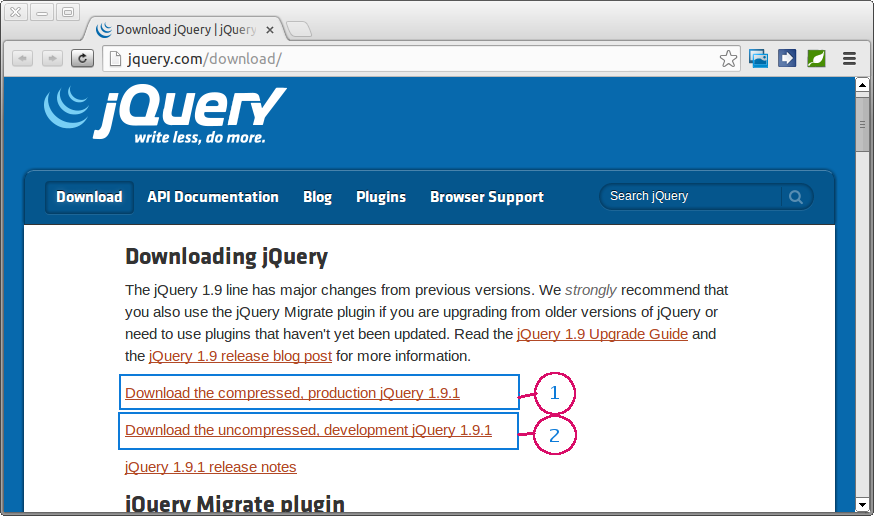
\includegraphics[width=0.75\textwidth]{figure/js-jquery.png}
\end{figure}
\newpage
& 嵌入方法
\begin{lstlisting}[tabsize=8, basicstyle=\small\tt, language=JavaScript, numbers=none]
<script type="text/javascript" src="jquery.js"></script>
\end{lstlisting}
& 使用托管版本
\begin{lstlisting}[tabsize=8, basicstyle=\small\tt, language=JavaScript, numbers=none]
<script type="text/javascript" 
src=" http://ajax.googleapis.com/ajax/libs/jquery/1.9.1/jquery.min.js "></script>
\end{lstlisting}
\end{easylist}
\end{frame}



\subsection{8.2 JavaScript的测试方法}

\begin{frame}[fragile]{8.2 JavaScript的测试方法}
\begin{easylist} \easyitem
& 与网页的关联测试方法
& 在页面加载之后运行JavaScript
& 浏览器内置的JavaScript控制台
\end{easylist}
\end{frame}


\subsubsection{8.2.1 与网页的关联测试方法}
\begin{frame}[fragile]{8.2.1 与网页的关联测试方法}
\begin{easylist} \easyitem
& 编写JavaScript脚本文件,并保存到以.js结尾的文件中,然后通过HTML语言中script标记的src属性进行关联
& 在<script>标记的开始和结束之间,直接嵌入JavaScript脚本
& 考虑二者的优缺点
\end{easylist}
\end{frame}


\begin{frame}[fragile]{示例}
\begin{lstlisting}[tabsize=8, basicstyle=\small\tt, language=HTML]
<html>
    <head>
        <title>JavaScript DEMO</title>
        <script type="text/javascript" src="jquery.js"></script>
        <script type="text/javascript">
            $(document).ready(function() {
                alert('hello world');
            });
        </script>
    </head>
    <body>
        <h1>JavaScript Test</h1>
    </body>
</html>
\end{lstlisting}
\end{frame}


\subsubsection{8.2.2 在页面加载之后运行JavaScript}
\begin{frame}[fragile]{8.2.2 在页面加载之后运行JavaScript}
\begin{easylist} \easyitem
& JavaScript默认在网页中的添加位置立即加载运行
&& 问题
&& 难度
& jQuery的实现方式
\begin{lstlisting}[tabsize=8, basicstyle=\small\tt, language=JavaScript, numbers=none]
$(document).ready(function() {
    //将想在网页加载完毕后再运行的代码放在此处…
});
\end{lstlisting}
\end{easylist}
\end{frame}


\subsubsection{8.2.3 利用浏览器内置的JavaScript控制台}
\begin{frame}[fragile]{8.2.3 利用浏览器内置的JavaScript控制台}
\begin{easylist} \easyitem
& Firefox
&& “Tools” $\rightarrow$ “Web Developer” $\rightarrow$ “Web Console”
&& CTRL+SHIFT+K
& CHROME
&& “Tools” $\rightarrow$ “JavaScript Console”
&& CTRL+SHIFT+J
& OPERA
&& “Developer Tools” $\rightarrow$ “Web Inspector”
&& CTRL+SHIFT+I
& IE
&& “Tools” $\rightarrow$ “F12 Developer Tools”
&& F12
\end{easylist}
\end{frame}


\begin{frame}[fragile]{Google Chrome的JavaScript控制台}
\begin{figure}
    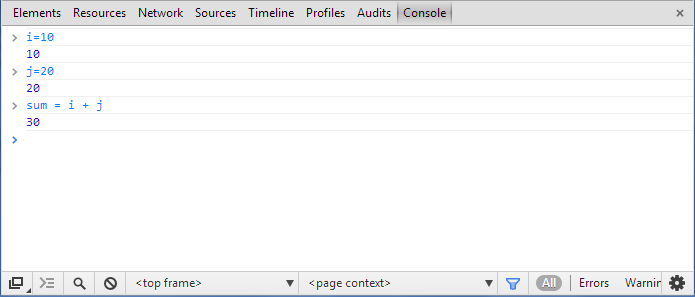
\includegraphics[width=0.9\textwidth]{figure/js-chrome-console.png}
\end{figure}
\end{frame}



\subsection{8.3 JavaScript的变量和常量}

\begin{frame}[fragile]{8.3 JavaScript的变量和常量}
\begin{easylist} \easyitem
& 数据类型
& 变量的声明和赋值
& 变量的作用域
& 常量
\end{easylist}
\end{frame}


\subsubsection{8.3.1 数据类型}
\begin{frame}[fragile]{8.3.1 数据类型}
\begin{figure}
    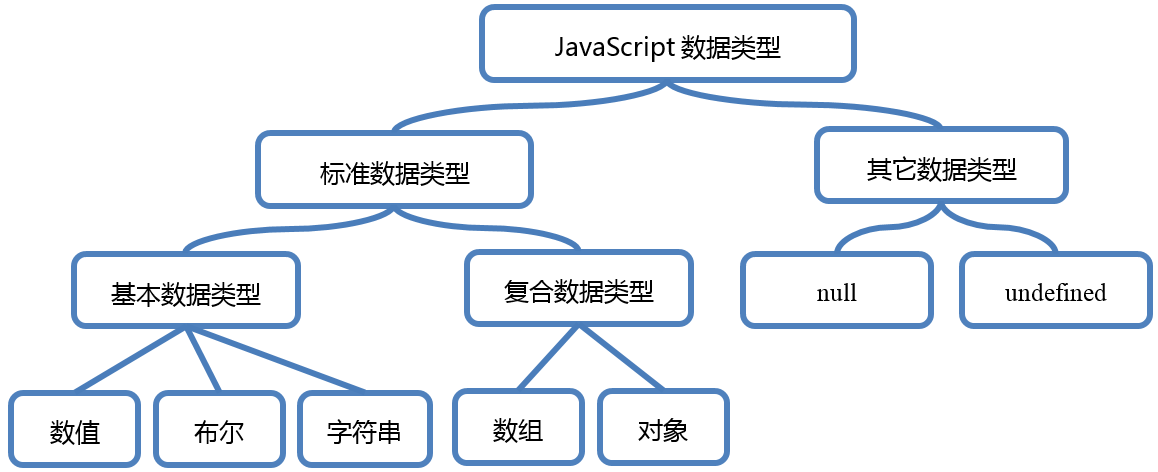
\includegraphics[width=1.0\textwidth]{figure/js-datatype.png}
\end{figure}
\end{frame}


\begin{frame}[fragile]{利用控制台查看数据类型}
\begin{figure}
    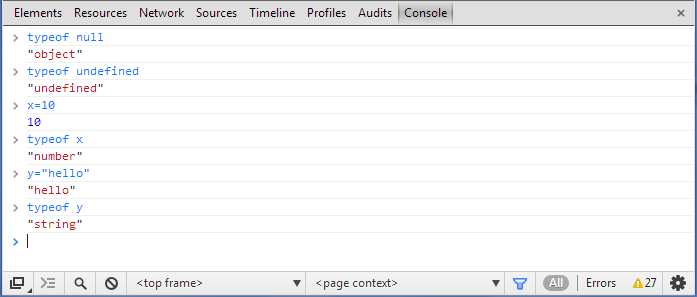
\includegraphics[width=1.0\textwidth]{figure/js-datatype2.png}
\end{figure}
\end{frame}


\subsubsection{8.3.2 变量的声明和赋值}
\begin{frame}[fragile]{8.3.2 变量的声明和赋值}
\begin{easylist} \easyitem
& 变量声明
\begin{lstlisting}[tabsize=8, basicstyle=\small\tt, language=JavaScript, numbers=none]
var userName;
\end{lstlisting}
& 变量赋值
\begin{lstlisting}[tabsize=8, basicstyle=\small\tt, language=JavaScript, numbers=none]
username="李白";
\end{lstlisting}
& 声明和赋值同时进行
\begin{lstlisting}[tabsize=8, basicstyle=\small\tt, language=JavaScript, numbers=none]
var userName="李白";
\end{lstlisting}
\end{easylist}
\end{frame}


\subsubsection{8.3.3 变量的作用域}
\begin{frame}[fragile]{8.3.3 变量的作用域}
\begin{easylist} \easyitem
& 全局变量
&& 在函数之外声明的变量
& 局部变量
&& 在函数之中声明的变量
& 局部变量对全局变量具有覆盖作用
& 考虑以下代码的输出结果:
\begin{lstlisting}[tabsize=8, basicstyle=\small\tt, language=JavaScript]
var a = 6;
function myfunction(){
    var a = 7;
    var b = 8;
    return a+b;
}
console.info(myfunction());
\end{lstlisting}
\end{easylist}
\end{frame}


\subsubsection{8.3.4 常量}
\begin{frame}[fragile]{8.3.4 常量}
\begin{easylist} \easyitem
& 不变的量,用关键字const来声明
\begin{lstlisting}[tabsize=8, basicstyle=\small\tt, language=JavaScript, numbers=none]
const A = 10;
const B = .314;
\end{lstlisting}
& 常量类型
&& 数字常量
&& 非数字NaN(Not A Number)
&& 布尔常量:true、false
&& 字符串
&& 转义字符
&&& $\backslash$b(退格)、$\backslash$f(换页)、$\backslash$n(换行)、$\backslash$r(回车)、$\backslash$t(跳格)、$\backslash$’(单引号)、$\backslash$"(双引号)
\end{easylist}
\end{frame}



\subsection{8.4 JavaScript的基本语句}

\begin{frame}[fragile]{8.4 JavaScript的基本语句}
\begin{easylist} \easyitem
& 注释语句
& 条件语句
& 循环语句
\end{easylist}
\end{frame}


\subsubsection{8.4.1 注释语句}
\begin{frame}[fragile]{8.4.1 注释语句}
\begin{lstlisting}[tabsize=8, basicstyle=\small\tt, language=JavaScript]
//这一行是注释内容
/*这里
*也是注释内容
*/
\end{lstlisting}
\end{frame}


\subsubsection{8.4.2 条件语句}
\begin{frame}[fragile]{8.4.2 条件语句}
\begin{easylist} \easyitem
& 条件运算符
&& 比较运算符
&&& >, >=, <, <=, ==, !=
&& 逻辑运算符
&&& \&\&, ||, !
& if语句
\end{easylist}
\end{frame}


\begin{frame}[fragile]{if语句}
\begin{lstlisting}[tabsize=8, basicstyle=\small\tt, language=JavaScript]
var hour = 20;
if (hour == 20) {
    alert("Now is 20 o’clock.");
}
\end{lstlisting}
\end{frame}


\begin{frame}[fragile, allowframebreaks]{if-else-else if语句}
\begin{lstlisting}[tabsize=8, basicstyle=\small\tt, language=HTML]
<html>
    <head>
        <title>IF DEMO</title>
        <meta http-equiv="Content-Type" content="text/html;charset=utf-8"/>
    </head>
    <body>
        <h1>条件语句测试</h1>
        <script type="text/javascript">
            var d = new Date();  //get current date and time
            var hour = d.getHours();
            var msg;

            if((hour>=7) && (hour<12)) {
                msg = '上午';
            } else if((hour>=12) && (hour<18)){
                msg = '下午';
            } else if((hour>=18) && (hour<22)) {
                msg = '晚上';
            } else {
                msg = '夜间';
            }

            document.write('现在是:' + msg);
        </script>
    </body>
</html>
\end{lstlisting}
\end{frame}


\subsubsection{8.4.3 循环语句}
\begin{frame}[fragile]{8.4.3 循环语句}
\begin{easylist} \easyitem
& for
\begin{lstlisting}[tabsize=8, basicstyle=\small\tt, language=JavaScript, numbers=none]
for (初始变量; 循环条件; 变量更新){
    循环主体语句;
}
\end{lstlisting}
& while
\begin{lstlisting}[tabsize=8, basicstyle=\small\tt, language=JavaScript, numbers=none]
while (循环条件){
    循环主体语句;
}
\end{lstlisting}
& break \& continue
\end{easylist}
\end{frame}


\begin{frame}[fragile, allowframebreaks]{循环语句示例}
\begin{lstlisting}[tabsize=8, basicstyle=\small\tt, language=HTML]
<html>
    <head>
        <title>LOOP DEMO</title>
        <meta http-equiv="Content-Type" content="text/html;charset=utf-8"/>
    </head>
    <body>
        <h1>条件语句测试</h1>
        <script type="text/javascript">
            var i=0, n=30, sum=0;
            var lastNumber = 0;
            while(i < n){
                if(i%2 == 0){
                    i++;
                    continue;
                } else {
                    sum = sum + i;
                    lastNumber = i;
                    i++;
                }
                if(i >= 50) break;
            }
            document.write('1+3+5+...+' + lastNumber + '=' + sum);
        </script>
    </body>
</html>
\end{lstlisting}
\end{frame}


\subsection{8.5 函数和数组}

\begin{frame}[fragile]{8.5 函数和数组}
\begin{easylist} \easyitem
& 函数
& 数组
\end{easylist}
\end{frame}


\subsubsection{8.5.1 函数}
\begin{frame}[fragile, allowframebreaks]{8.5.1 函数}
\begin{easylist} \easyitem
& 创建函数
\begin{lstlisting}[tabsize=8, basicstyle=\small\tt, language=JavaScript, numbers=none]
function 函数名称(参数列表) {
    函数内部的语句段
}
\end{lstlisting}
& 例子
\begin{lstlisting}[tabsize=8, basicstyle=\small\tt, language=JavaScript]
//函数示例1:函数中包括了alert这个内置的弹出警告框函数
function welcome () {
    alert ( "hello,this is a function!");
} 

//函数示例2:对a、b两个参数进行求和,并用return语句返回结果
function sum ( a,b) {
    return a+b;
}
\end{lstlisting}

& 字面量方式创建函数
\begin{lstlisting}[tabsize=8, basicstyle=\small\tt, language=JavaScript, numbers=none]
var变量名称 = function 可选函数名称(函数参数){语句段};
\end{lstlisting}
& 例子
\begin{lstlisting}[tabsize=8, basicstyle=\small\tt, language=JavaScript]
var test = function(){
    alert("hello world");
}
test();
\end{lstlisting}
\end{easylist}
\end{frame}

\begin{frame}[fragile]{函数参数}
\begin{easylist} \easyitem
& 形式参数(形参) vs 实际参数(实参)
&& 形式参数只是一个指代,而真正在调用中起作用的是实参
& 例子
\begin{lstlisting}[tabsize=8, basicstyle=\small\tt, language=JavaScript]
function plus (a,b) { //这里a,b是形式参数
    return a+b;
}
plus (3, 5);  //将两个数字作为实参传入
plus (plus(1,2) ,plus(2,3));  //将两个函数作为实参传入
\end{lstlisting}
& Arguments
\end{easylist}
\end{frame}


\begin{frame}[fragile]{函数调用与返回}
\begin{lstlisting}[tabsize=8, basicstyle=\small\tt, language=JavaScript]
function add (x,y){
    return x+y;
}
alert (add(3,9));
\end{lstlisting}
\end{frame}


\subsubsection{8.5.2 数组}
\begin{frame}[fragile]{8.5.2 数组}
\begin{easylist} \easyitem
& 创建数组
\begin{lstlisting}[tabsize=8, basicstyle=\small\tt, language=JavaScript]
var base = [1,2,3,4,5,6,7,8];
var table = [[1,2,3,4],[5,6,7,8],[9,10,11,12]];  //此处构造了一个二维数组
\end{lstlisting}

& 访问和修改
\begin{lstlisting}[tabsize=8, basicstyle=\small\tt, language=JavaScript]
var base = [1,2,3,4,5,6,7,8,9];
base[0] = 10;
base[1] = 20;
for (var i=0;i<base.length;i++)
    base[i]++;
console.info(base);
\end{lstlisting}
\end{easylist}
\end{frame}



\subsection{8.6 对象}

\begin{frame}[fragile]{8.6 对象}
\begin{easylist} \easyitem
& 创建对象
& 属性和方法
& 基本类型和引用类型
& 原型与继承
& 类方法
\end{easylist}
\end{frame}


\subsubsection{8.6.1 创建对象}
\begin{frame}[fragile]{8.6.1 创建对象}
\begin{easylist} \easyitem
& 对象类型
&& Object
&& Function(函数对象)
&& Array(数组对象)
&& Date
&& Math
&& RegExp(正则表达式)
&& Error(错误)
&& 字符串、布尔、数值的包装对象:String、Boolean、Number
\end{easylist}
\end{frame}


\begin{frame}[fragile]{通过new构造对象}
\begin{lstlisting}[tabsize=8, basicstyle=\small\tt, language=JavaScript]
var num=new Object();//自定义一个Object对象的实例并命名为num
num.x=1;
num.y=2;  //为num对象设置两个属性x和y,并分别赋值为1和2
var z=new Array(3);  //定义一个长度为3的数组对象z
var a=new Array (1,2,3,4); //定义一个数组对象a并设定前4个元素为1、2、3、4
var b=new function(){
    alert("hello world");
}  //定义一个函数对象b
\end{lstlisting}
\end{frame}


\begin{frame}[fragile]{通过字面量构造对象}
\begin{lstlisting}[tabsize=8, basicstyle=\small\tt, language=JavaScript]
obj_1 = {
    x: "h1",
    y: function () {
        alert("Hello world!");
    }
};
obj_2 = {
    z: [1,2,3,4],
    add: function(a,b) {
        return a+b;
    }
};
\end{lstlisting}
\end{frame}



\subsubsection{8.6.2 属性和方法}
\begin{frame}[fragile]{8.6.2 属性和方法}
\begin{lstlisting}[tabsize=8, basicstyle=\small\tt, language=JavaScript]
var obj = {};
obj.color = "red";
obj.text = "hello";
obj.work = function(worker){
    console.info(worker + " is working!");
};
\end{lstlisting}
\end{frame}


\subsubsection{8.6.3 基本类型和引用类型}
\begin{frame}[fragile, allowframebreaks]{8.6.3 基本类型和引用类型}
\begin{easylist} \easyitem
& 基本类型
&& 指数值、字符串、布尔值等这类原始值
& 引用类型
&& 指对象类型
\newpage
& 例子
\begin{lstlisting}[tabsize=8, basicstyle=\small\tt, language=JavaScript]
var a = 6;
var b = a;
var b = 7;//此时b的值为7,a的值仍为6
console.info("a=" + a + ", b=" + b);
var oneday= new Date (2050,1,1);
var c = oneday;
c.setDate(11);
oneday.getDate();//此时变量c和oneday的日期的天数均变为11
console.info("oneday.getDate()=" + oneday.getDate() + ", c.getDate()=" + c.getDate());
\end{lstlisting}
&& 思考:输出结果为?
\end{easylist}
\end{frame}


\subsubsection{8.6.4 原型与继承}
\begin{frame}[fragile, allowframebreaks]{8.6.4 原型与继承}
\begin{easylist} \easyitem
& JavaScript借助于原型(prototype)实现继承
&& 把prototype看作是一个模版,新创建的自定义对象则是这个模版(prototype)的一个拷贝
& 例子
\begin{lstlisting}[tabsize=8, basicstyle=\small\tt, language=JavaScript]
function Animal(name, age) {
    this.name = name;
    this.age = age;
}
Animal.prototype = {
    getName: function(){
        return this.name;
    },
    getAge: function(){
        return this.age;
    }
}
var tom = new Animal("Tom Cat", 2);
console.info(tom.getName() + " is " + tom.getAge() + " years old.");
\end{lstlisting}
& 每一个对象都有相应的原型
& prototype属性默认初始化为一个对象
\end{easylist}
\end{frame}



\subsubsection{8.6.5 类方法}
\begin{frame}[fragile, allowframebreaks]{8.6.5 类方法}
\begin{easylist} \easyitem
& 实例方法、原型方法和类方法
& 例子
\begin{lstlisting}[tabsize=8, basicstyle=\small\tt, language=JavaScript]
function Animal(name) {
    this.name=name;
    //以下定义的introduce 为实例方法
    this.introduce=function(){
        console.info("I am " + this.name);
    }
}

//类方法
Animal.run = function(){
    console.info("I can run");
}

//原型方法
Animal.prototype.introduceInChinese=function(){
    console.info("我是"+this.name);
}

//测试
var tom =new Animal("Tom Cat");
tom.introduce();
Animal.run(); //注意:类方法只能通过类名称调用,不能通过实例调用,如tom.run()
tom.introduceInChinese();
\end{lstlisting}
\end{easylist}
\end{frame}



\subsection{8.7 浏览器对象模型BOM}

\begin{frame}[fragile]{8.7 浏览器对象模型BOM}
\begin{easylist} \easyitem
& \em{Widow}
& \em{Document}
& Navigator
& Location
& Screen
& History
\end{easylist}
\end{frame}


\begin{frame}[fragile]{Window}
\begin{easylist} \easyitem
& window是全局对象,每个窗口(包括浏览器窗口和框架窗口)都对应于一个Window对象
& 引用方式
&& window.属性名称或方法名
&& 当访问当前窗口的window对象,可以省略window
&& window对象是代码在浏览器中解释时的全局对象,当运行环境不是浏览器时,window对象不存在
\end{easylist}
\end{frame}


\begin{frame}[fragile]{常见的Window对象的属性和方法}
\begin{table}[!hbp] 
\begin{tabular}{l|l}
\Xhline{1.3pt}
属性/方法名称 & 描述  \\ \Xhline{1.3pt}
document & 返回浏览器内置的Document对象 \\ \hline
navigator & 返回浏览器内置的Navigator对象 \\ \hline
location & 返回浏览器内置的Location对象 \\ \hline
history & 返回浏览器内置的History对象 \\ \hline
screen & 返回浏览器内置的Screen对象 \\ \hline
name & 设置或返回窗口的名称 \\ \hline
open() & 创建一个新的浏览器窗并载入指定的url \\ \hline
close() & 关闭一个浏览器窗口 \\ \hline
alert() & 弹出一个消息框 \\ \hline
confirm() & 弹出一个确认框 \\ \hline
prompt() & 弹出一个提示框 \\ \hline
\end{tabular}
\end{table}
\end{frame}


\begin{frame}[fragile]{常见的Document对象的属性和方法}
\begin{table}[!hbp] 
\begin{tabular}{l|l}
\Xhline{1.3pt}
属性/方法名称 & 描述  \\ \Xhline{1.3pt}
body & 访问文档的body元素 \\ \hline
domain & 返回当前文档的域名 \\ \hline
title & 返回当前文档的标题 \\ \hline
URL & 返回当前文档的URL \\ \hline
referrer & 返回载入当前文档的原文档的URL \\ \hline
getElementById() & 返回对拥有指定 id 的第一个对象的引用 \\ \hline
getElementsByTagName() & 返回带有指定标签名称的对象集合 \\ \hline
write() & 向当前文档写入HTML表达式或JS代码 \\ \hline
writeln() & 等同于write(),但在输出后会添加换行符 \\ \hline
\end{tabular}
\end{table}
\end{frame}


\begin{frame}[fragile]{练习}
\begin{easylist} \easyitem
& 通过JavaScript控制台获取网页http://www.ruc.edu.cn/中的所有链接
\end{easylist}
\end{frame}



\subsection{8.8 定时器}

\begin{frame}[fragile]{8.8 定时器}
\begin{easylist} \easyitem
& 一次性定时器
&& 设置:setTimeout(f, milliseconds);
&& 取消:clearTimeout(timer);
& 重复定时器
&& 设置:setInterval(f, milliseconds);
&& 取消:clearInterval(timer);
\end{easylist}
\end{frame}

\begin{frame}[fragile]{定时器示例}
\begin{lstlisting}[tabsize=8, basicstyle=\small\tt, language=HTML]
<html>
    <head>
        <title>setTimeout DEMO</title>
        <script type="text/javascript" src="jquery.js"></script>
        <script type="text/javascript">
            $(document).ready(function() {
                function onTimer( ){
                    alert("DING DING");
                };
                var timer = setTimeout(onTimer, 2000);
            });
        </script>
    </head>
    <body>
        <h1>setTimeout DEMO</h1>
    </body>
</html>
\end{lstlisting}
\end{frame}



\begin{frame}
\begin{center}
    \Huge END
\end{center}
\begin{figure}
    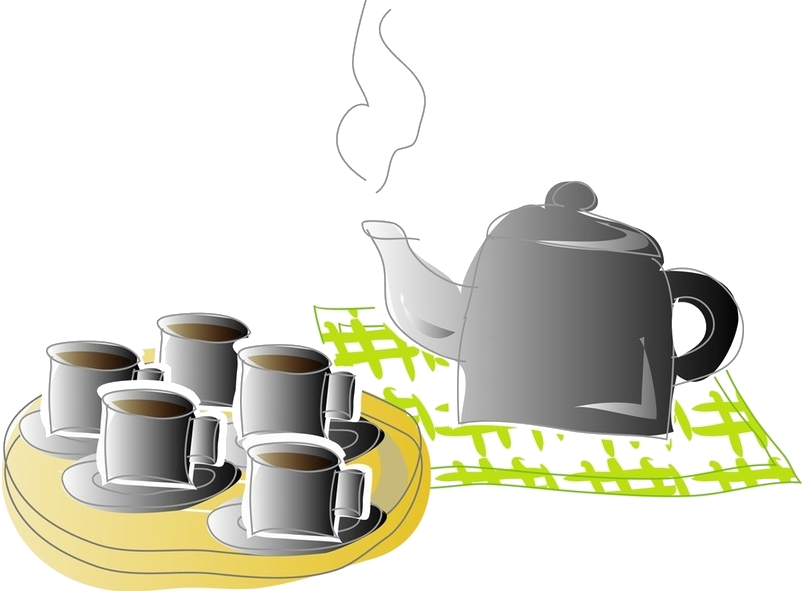
\includegraphics[width=0.75\textwidth]{figure/relax.png}
\end{figure}
\end{frame}
